% ------------------------------------------------------------------------------
% Este fichero es parte de la plantilla LaTeX para la realización de Proyectos
% Final de Grado, protegido bajo los términos de la licencia GFDL.
% Para más información, la licencia completa viene incluida en el
% fichero fdl-1.3.tex

% Copyright (C) 2012 SPI-FM. Universidad de Cádiz
% ------------------------------------------------------------------------------

Este capítulo trata sobre todos los aspectos relacionados con la implementación del sistema en código, haciendo uso de un determinado entorno tecnológico.

\section{Entorno de Construcción}
En esta sección se debe indicar el marco tecnológico utilizado para la construcción del sistema: entorno de desarrollo (IDE), lenguaje de programación, herramientas de ayuda a la construcción y despliegue, control de versiones, repositorio de componentes, integración contínua, etc.

Para desarrollar este proyecto hemos usado:

\begin{itemize}
	\item \href{http://www.codeigniter.com/}{CodeIgniter} [\url{http://www.codeigniter.com/}]
	\item \href{https://secure.php.net/}{PHP} [\url{https://secure.php.net/}]
	\item HTML[\url{https://es.wikipedia.org/wiki/HTML}]
	\item \href{https://www.mysql.com/}{MYSQL} [\url{https://www.mysql.com/}]
	\item \href{https://forja.rediris.es/}{Forja Rediris} [\url{https://forja.rediris.es/}]
	\item \href{http://tortoisesvn.net/}{Tortoise SVN} [\url{http://tortoisesvn.net//}]
	\item \href{https://www.mozilla.org/es-ES/}{Firefox} [\url{https://www.mozilla.org/es-ES/}]
	\item \href{http://www.latex-project.org/}{LaTeX} [\url{http://www.latex-project.org/}]
	\item \href{http://www.texstudio.org/}{TeXtudio} [\url{http://www.texstudio.org/}]
	\item \href{http://dia-installer.de/index.html.es}{Dia} [\url{http://dia-installer.de/index.html.es}]	
\end{itemize}

\section{Código Fuente}
Organización del código fuente, describiendo la utilidad de los diferentes ficheros y su distribución en paquetes o directorios. Asimismo, se incluirá algún extracto significativo de código fuente que sea de interés para ilustrar algún algoritmo o funcionalidad específica del sistema.\\

Se ha usado una estructura modelo vista controlador, de forma que al analizar inicialmente el sistema, pude ver que en la carpeta de vista guardaremos las interfaces, en la de modelos guardaremos los objetos donde se definen todas las funciones y en la carpeta de controladores guardaremos los controladores, que hacen posible que vistas y modelos interactúen entre si.\\

También me gustaría destacar el algoritmo de barajado aleatorio usado para la preasignación de ediciones a los alumnos.\\
Fuente: 
\href{https://es.wikipedia.org/wiki/Algoritmo_Fisher-Yates}{Wikipedia: Algoritmo Fisher-Yates}

Otra cosa a destacar es que con el antiguo esquema de la base de datos, al realizarse una re-evaluación, esta no era tratada de forma especial, y contaba como si fuese una evaluación normal de una edición.
Gracias a la nueva distribución de la base de datos se ha solventado ese problema, manteniendo a su vez la compatibilidad con otros sistemas como StatMediaWiki o CleverFigures

\section{Scripts de Base de datos}
Organización del código fuente, describiendo la utilidad de los diferentes ficheros y su distribución en paquetes o directorios. Asimismo, se incluirá el script de algún disparador o un procedimiento almacenado, que sea de interés para ilustrar algún aspecto concreto de la gestión de la base de datos.

La mayoría de funciones para manejar las bases de datos se encuentran en los modelos del sistema.\\

Como se ha mencionado anteriormente, al modificar la estructura de la base de datos del sistema (ver [Fig.6.1] y [Fig.6.2] a continuación) se ha conseguido solventar algunas debilidades de la versión anterior, así como implementar mejoras como las ráfagas y las preasignaciones, para las cuales es necesario que las bases de datos de AssessMediaWiki y MediaWiki se intercomuniquen, ese proceso se puede observar con mas detenimiento en el modelo de ejercicios de evaluación.

\clearpage

\begin{figure}
	\centering
	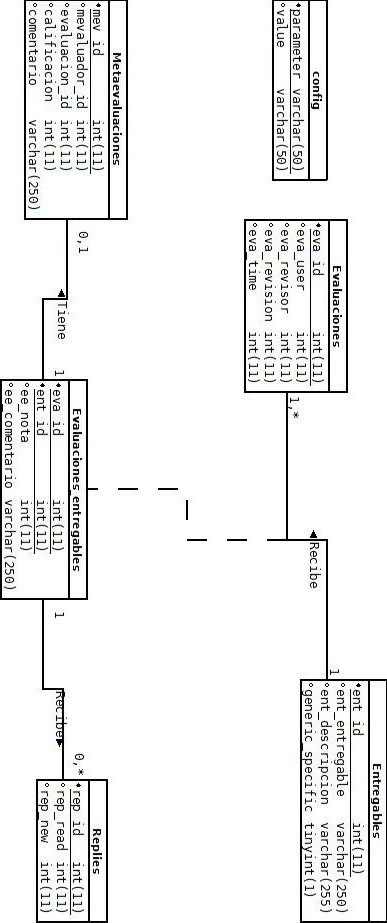
\includegraphics[width=0.6\textwidth]{db1girada.jpg}
	\caption{Diagrama de la base de datos de AMW 1.0.}
\end{figure}

\begin{figure}
	\centering
	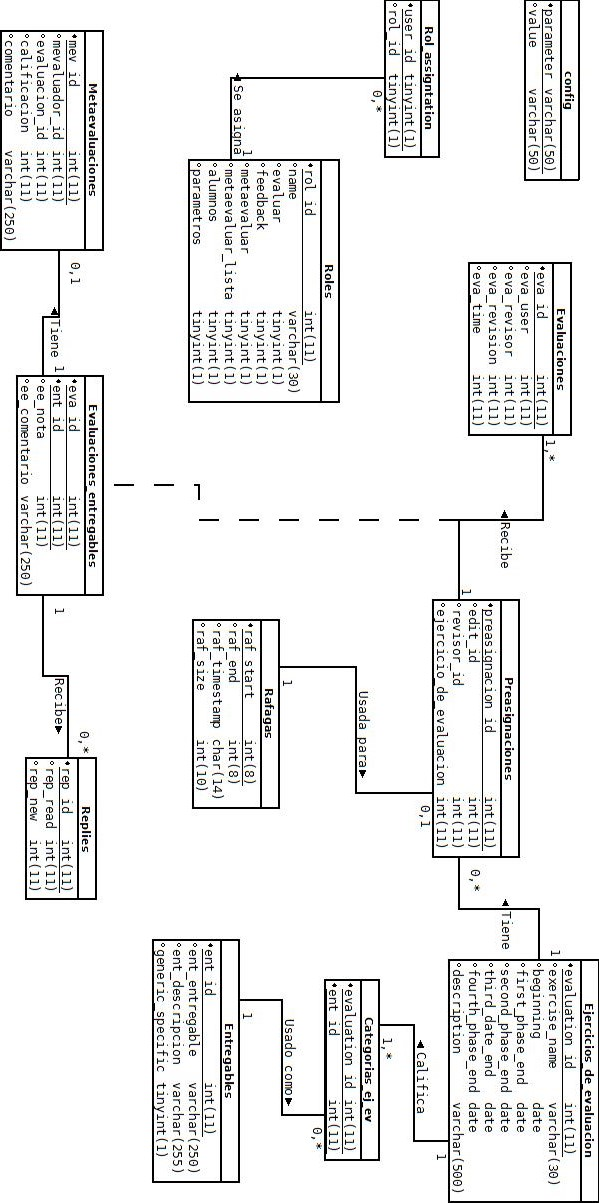
\includegraphics[width=0.6\textwidth]{db2girada.jpg}
	\caption{Diagrama de la base de datos de AMW 2.0.}
\end{figure}

\clearpage